\documentclass[12pt]{article}

\usepackage[utf8x]{inputenc}
\usepackage[spanish,es-noshorthands]{babel}

\usepackage{amssymb,amsmath,amsthm,amsfonts}
\usepackage{calc}
\usepackage{graphicx}
\usepackage{subfigure}
\usepackage{gensymb}
\usepackage{natbib}
\usepackage{url}
\usepackage[utf8x]{inputenc}
\usepackage{amsmath}
\usepackage{graphicx}
\graphicspath{{images/}}
\usepackage{parskip}
\usepackage{fancyhdr}
\usepackage{vmargin}
\usepackage{verbatim}
\setmarginsrb{3 cm}{2.5 cm}{3 cm}{2.5 cm}{1 cm}{1.5 cm}{1 cm}{1.5 cm}

\title{Tu titulo}					% Titulo
\author{Tu nombre}					% Autor
\date{\today}						% Fecha


\makeatletter
\let\thetitle\@title
\let\theauthor\@author
\let\thedate\@date
\makeatother

\pagestyle{fancy}
\fancyhf{}
\rhead{\theauthor}
\lhead{\thetitle}
\cfoot{\thepage}

\begin{document}

\tableofcontents
\pagebreak

%%%%%%%%%%%%%%%%%%%%%%%%%%%%%%%%%%%%%%%%%%%%%%%%%%%%%%%%%%%%%%%%%%%%%%%%%%%%%%%%%%%%%%%%%

\section{Introducción.}

Los sistemas de control de plantas termosolares de receptor central son sistemas complejos que tienen entre sus objetivos concentrar energía solar reflejada por el campo de helióstatos en una serie de puntos. Obtener una medida de la radiación reflejada en un punto del receptor es una tarea complicada debido a la dificultad de medir directamente dicha radiación concentrada. Este trabajo plantea como objetivo general el aproximarse a esta medida mediante la utilización del tratamiento digital de imágenes de la proyección de la radiación solar concentrada por un helióstato.
La obtención en tiempo real de parámetros matemáticos obtenidos del análisis de dichas imágenes, así como su correlación con variables físicas, permitirán una estimación óptima de la distribución de radiación solar concentrada por un helióstato en un receptor. Esta estimación de la distribución podría ser aplicada a la proyección de un conjunto de helióstatos, así como utilizada en tareas diarias de operación y mantenimiento de un campo de helióstatos.

\section{Objetivos y justificación.}

Este proyecto tiene como objetivo fundamental obtener los parámetros matemáticos de una imagen de ejemplo de la proyección de la radiación solar reflejada por un helióstato de la Plataforma Solar de Almería (CIEMAT) sobre una diana. Con dichos parámetros se construirá un estimador de la cantidad de radiación solar concentrada.
Para ello se utilizarán como herramientas la librería de código abierto OpenCV a través de su interfase en lenguaje Python/C/C++ y sobre el sistema operativo UNIX/Linux. Se utilizarán las primitivas que dicho sistema ofrece para obtener la medida del tiempo de cómputo de cada parámetro ante diferentes configuraciones de computador (concurrencia, paralelismo, ...). \cite{OpenCVWebSite} \cite{SALWebSite} \cite{IEEEXploreWebSite}

\section{Helióstatos.}

Un helióstato es un conjunto de espejos que establecen una superficie grande y se mueven sobre uno o dos ejes, normalmente en montura acimutal, lo que permite, con los movimientos apropiados, mantener el reflejo de los rayos solares que inciden sobre él, se fijen en todo momento en un punto o superficie. Haciendo esto, los rayos que refleja el helióstato pueden ser dirigidos hacia un solo punto (o superficie) durante todo el día.

Se utilizan fundamentalmente en observaciones astronómicas para mantener fija la imagen del Sol o de un astro sobre el aparato de observación, en cuyo caso suelen ser de pequeñas dimensiones. La aplicación de este proyecto es en el uso de centrales solares termoeléctricas para concentrar la energía solar sobre el receptor, y conseguir así altas temperaturas. Estos helióstatos suelen ser grandes, llegando a tener más de 120 m2.

En experimentación y pruebas de materiales a altas temperaturas, un conjunto suficientemente alto de helióstatos puede concentrar los rayos solares hasta conseguir temperaturas de más de 2000 ºC.

Los primeros helióstatos considerados como elementos industriales se desarrollaron a los inicios de la década de los ochenta para las plantas experimentales termosolares de receptor central, con el propósito de probar la viabilidad de la energía solar térmica en los procesos de producción de electricidad a escala industrial. Las figuras 1 y 2 muestran, respectivamente, un campo de helióstatos y un helióstato.

\section{Helióstato con sensor de reflexión.}

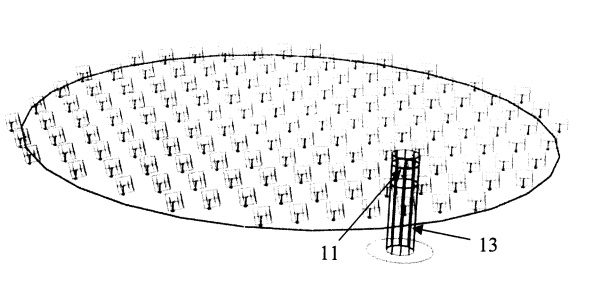
\includegraphics[width=\textwidth]{unnamed (1).jpg}
\cite{OepmWebSite}

Figura 1.

El helióstato con sensor de reflexión es un helióstato perteneciente a un campo solar que refleja los haces de luz que llegan a él dotado de un mecanismo de seguimiento solar. Se trata de una invención que pertenece dentro del área de la termotecnia, al campo de la producción de energía a partir de la radiación solar.

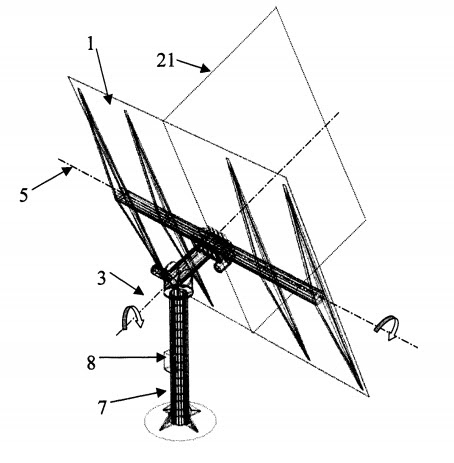
\includegraphics[width=\textwidth]{unnamed.jpg}
\cite{OepmWebSite}

Figura 2.

Desde mediados del siglo XX se vienen realizando investigaciones para intentar transformar esa energía en electricidad. Es por esto que se han desarrollado helióstatos que concentran haces de luz sobre un receptor central que contiene un fluido logran alcanzar temperaturas suficientes como para producir grandes cantidades de vapor de agua que genera electricidad a través de una turbina, normalmente en un ciclo de Rankine.

\cite{GstriatumWebSite} \cite{EcuRedWebSite}

\section{Funcionamiento de la central solar de receptor central o de tipo torre.}

Una central solar de tipo torre central, está formada por un campo de helióstatos que reflejan la luz del sol y concentran los haces reflejados en una caldera situada sobre una torre de gran altura.

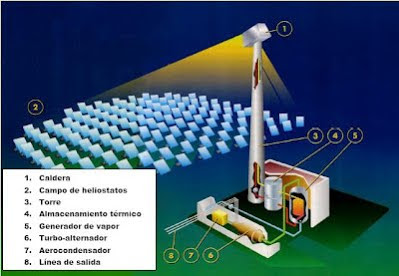
\includegraphics[width=\textwidth]{unnamed (2).jpg}

En la caldera, el aporte calorífico obtenido es transferido a un fluido térmico. Dicho fluido es conducido hacia un generador de vapor donde transfiere el calor a agua se convierte en vapor, y acciona los álabes del grupo turbina-alternador generando energía eléctrica. El vapor es posteriormente condensado en un aerocondensador para repetir el ciclo.

La producción de una central térmica depende de una serie de factores:

La cantidad de horas que este fluido esté expuesto al sol.
El lugar donde la fábrica esté situada.
La calidad de los depósitos de almacenamiento del fluido.

La energía producida, después de ser transformada, es transportada mediante líneas a la red general. \cite{LuciaRinconWebSite}

La potencia de la torre central va de los 10 a los 200 MW, habiéndose instalado ya diferentes plantas comerciales.

Su buen funcionamiento para obtener el máximo aprovechamiento depende de la latitud y climatología (situación geográfica) a la que está sometida, así como los procedimientos de mantenimiento, operación y control de la planta.

Hay fundamentalmente dos tipos de configuración: una en la que los helióstatos rodean completamente a la torre central, y otra en la que los helióstatos están colocados al norte o sur de la torre.

BENEFICIOS DE LA TORRE CENTRAL:
Conforme se haya hecho la inversión y la instalación, ya no generará gastos mayores, el único será el del mantenimiento.
No requiere el uso de combustibles, lo que evita el riesgo de almacenar combustibles.
No contamina, ya que la energía solar no produce desechos, residuos ni vapores.

INCONVENIENTES:
Se debe de instalar en lugares en donde la radiación del sol sea durante el mayor tiempo posible durante todo el día.
Todo su sistema mecánico es más complejo que otros sistemas.
Se necesitan acumuladores de calor para poder usar este dispositivo para cuando no haya radiación.

En la turbina se genera la energía eléctrica, y de ahí pasa a un generador y un transformador y finalmente a una subestación; mientras que el vapor de agua pasa a un condensador y a un sistema de enfriamiento para posteriormente pasar por una bomba a la caldera donde el ciclo se repite. \cite{IgualadaWebSite} \cite{SoliclimaWebSite} \cite{ClaudioWebSite}

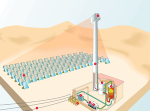
\includegraphics[width=\textwidth]{unnamed.png}
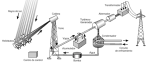
\includegraphics[width=\textwidth]{unnamed (1).png}

\section{Ejemplos de centrales de receptor central.}
\subsection{Plantas PS10 y PS20.}

PS10: La megatorre sevillana de la energía solar (y cómo funciona).

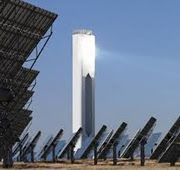
\includegraphics[width=\textwidth]{unnamed (4).jpg}
Planta Solúcar PS10
En Sanlúcar la Mayor, a 18 kilómetros de Sevilla, la empresa española Abengoa construyó una estación solar de generación de electricidad.

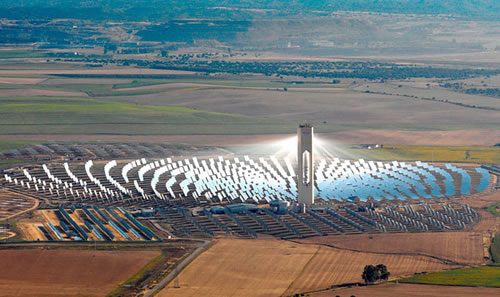
\includegraphics[width=\textwidth]{unnamed (3).jpg}
Campo de helióstatos y torre
Inaugurada en el año 2007, la PS10 fue la primera central solar termoeléctrica (de carácter comercial) de torre central y campo de helióstatos instalada en el mundo. Utiliza paneles de espejo para generar 11 megavatios.
Sólo PS10, PS20 y Solnovas, que se reúnen en la conocida como Planta Solúcar, operan comercialmente un total de 183 MW, produciendo energía anual equivalente a 94.000 hogares, y evitando así la emisión de más de 114.000 toneladas anuales de CO2 a la atmósfera.
La PS10 está formada por 624 helióstatos y una torre solar de 114 metros de altura. El campo de espejos o helióstatos refleja la luz solar sobre un receptor en la parte superior de la torre.

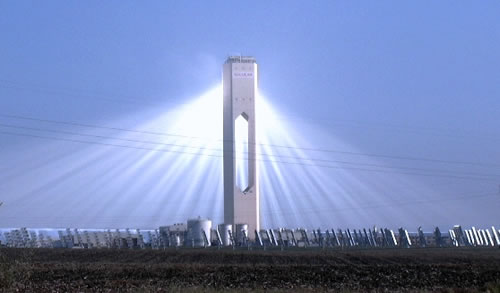
\includegraphics[width=\textwidth]{unnamed (5).jpg}
Esta torre se encuentra en el centro de la estación PS10 Solúcar. En la parte superior, el receptor solar consiste en una serie de paneles de tubos que operan a muy alta temperatura y por los que circula agua a presión. Este receptor se calienta por efecto de la luz solar y genera vapor saturado a 257 ºC. El vapor que se produce es almacenado parcialmente en unos tanques acumuladores para ser utilizado cuando no haya suficiente producción; el resto es enviado a accionar una turbina que genera la electricidad.

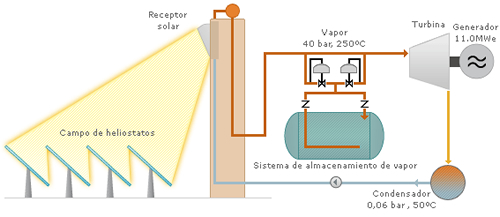
\includegraphics[width=\textwidth]{unnamed (7).jpg}

Esquema de funcionamiento
Los 624 helióstatos circundantes, cada uno con una superficie de 120 metros cuadrados, producen el reflejo para que el sistema pueda convertir alrededor del 17 por ciento de la energía de la luz solar en 11 megavatios de electricidad. Como punto de comparación, la planta PS20 (que se encuentra al lado) produce 20 MW de potencia mediante su torre de 160 metros de altura sobre un campo de 1.255 helióstatos.
Por lo tanto, esta planta funciona calentando agua con luz solar y, con el vapor generado, mueve turbinas para crear electricidad.

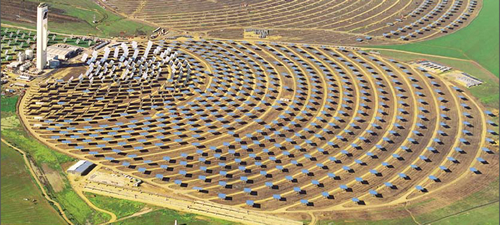
\includegraphics[width=\textwidth]{unnamed (6).jpg}

Campo y torre PS10
\cite{JonathanWebSite}



PS20.

La PS20 (Planta Solar 20) es una planta comercial situada al lado de la PS10.
A diferencia de la PS10, la PS20 cuenta con 85 hectáreas y con 1.255 helióstatos que reflejan los rayos al receptor situado en la parte superior de la torre de 160 metros de altura.
La PS20 dispone con un sistema de almacenamiento de 1 hora, con un receptor más eficiente y un sistema de control y operación mejor que le permiten producir 20 MW que abastecen a 10.000 hogares anualmente.

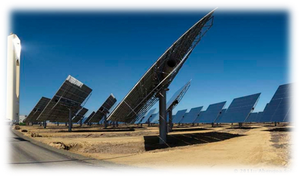
\includegraphics[width=\textwidth]{unnamed (2).png}
Helióstato PS10

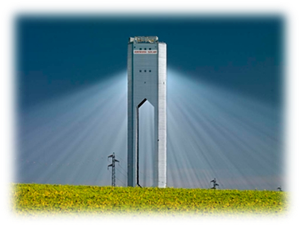
\includegraphics[width=\textwidth]{unnamed (3).png}
\cite{ValenticampderrosWebSite}

\subsection{Planta termosolar Gemasolar.}

Gemasolar es una planta de energía solar por concentración con sistema de almacenamiento térmico en sales fundidas situada en Sevilla, España. Es la primera a escala comercial en aplicar la tecnología de receptor de torre central y almacenamiento térmico en sales fundidas. La superficie de esta planta ocupa aproximadamente 158 hectáreas. Características:
Potencia eléctrica de 19,9 MW.
La producción neta esperada es de 110 GWh/año.
Capaz de suministrar energía limpia y segura que reduce en más de 50.000 toneladas al año de emisiones de CO2.
La planta está formada por:
2.650 heliostatos de 120 m2 que forman círculos concéntricos alrededor de la torre que disponen de un mecanismo que posiciona con precisión la superficie de los espejos.
Una torre que en lo alto se encuentra el receptor de haz de luz compuesto por paneles.
2 tanques: uno de sales frías y otro de sales calientes.
Un cambiador de calor; un generador y transformador.
Su funcionamiento se ilustra en la siguiente imagen:

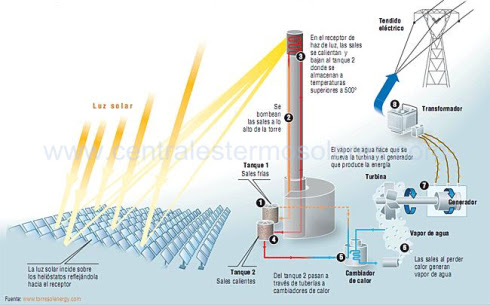
\includegraphics[width=\textwidth]{unnamed (8).jpg}

Tanque 1: Sales frías.
Se bombean las sales a lo largo de la torre.
En el receptor de haz de luz, las sales se calientan y bajan al tanque 2 donde se almacenan a temperaturas superiores a 500º.
Tanque 2: Sales calientes.
Cambiador de agua.
Las sales al perder calor generan vapor de agua.
El vapor de agua hace que se mueva la turbina y el generador que produce la energía.
Transformador. La energía pasa al tendido eléctrico.
La planta no solo funciona como una central solar sino también como una central térmica (cuando no hay luz solar) gracias a su sistema de concentración de sales y a partir de ahí también generar electricidad. También podemos decir que gracias a esto la planta asegura obtención de energía las 24 horas del días en situaciones de baja insolación, en las madrugadas y varios meses al año.
Es tal el éxito de la planta sevillana que muchos profesionales del sector buscan aplicar las energías limpias a las pequeñas urbanizaciones y así hacer posible su aplicación a la vida cotidiana. \cite{PonsWebSite}



\subsection{Planta termosolar de receptor central de Ivanpah.}

El Sistema de generación eléctrica solar Ivanpah es una planta termosolar concentrada en el desierto de Mojave. Está ubicado en la base de Clark Mountain en California, a través de la línea estatal desde Primm, Nevada. La planta tiene una capacidad bruta de 392 megavatios (MW). Su campo solar está formado por 173,500 helióstatos, de 14.05 m2 cada uno proyectando en tres torres la energía solar reflejada. La primera unidad del sistema se conectó a la red eléctrica en septiembre de 2013 para una prueba de sincronización inicial. La instalación abrió formalmente el 13 de febrero de 2014. En 2014, fue la estación de energía solar térmica más grande del mundo.
 
Los campos de espejos de helióstatos enfocan la luz solar en los receptores ubicados en torres de energía solar centralizadas. Los receptores generan vapor para accionar turbinas de vapor especialmente adaptadas.
 
Para la primera planta, se ordenó el mayor grupo generador de turbina de vapor con energía solar, con una turbina de recalentamiento de caja única Siemens SST-900 de 123 MW. Las plantas no tienen almacenaje, y calientan el vapor a 550 °C directamente en los receptores. La potencia total instalada de la planta de Ivanpah es de 377 MW eléctricos.
 
La instalación, con un costo de \$ 2.2 mil millones, fue desarrollada por BrightSource Energy y Bechtel. \cite{Wikipedia2WebSite}



\subsection{Proyecto de Google RE\textless C.}

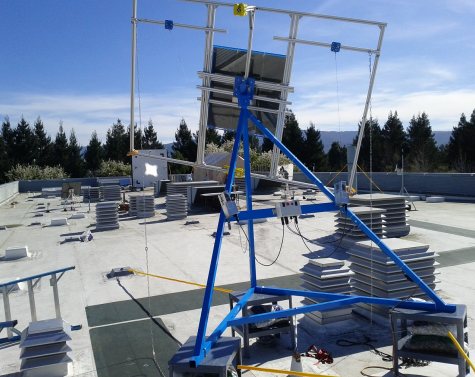
\includegraphics[width=\textwidth]{HeliostatoGoogle.png}

Un helióstato prototipo manteniendo la luz en el objetivo. \cite{Wikipedia3WebSite}

Introducción.

RE\textless C fue una iniciativa de Google para impulsar la innovación en energía renovable, con el objetivo de hacer que la energía renovable sea lo suficientemente barata para competir cara a cara con las centrales eléctricas de carbón.

Las plantas de energía solar concentradas (CSP) usan espejos o lentes para enfocar una gran cantidad de luz solar sobre un objetivo que absorbe calor, llamado receptor. El intercambiador de calor del receptor crea vapor a alta presión, que luego impulsa una turbina para alimentar un generador eléctrico. La refrigeración por agua en spray se utiliza normalmente para condensar el vapor.

La CSP modular de "torre de energía" utiliza un motor de turbina de gas más pequeño (Brayton) para realizar la conversión de energía. Los motores Brayton no necesitan refrigeración por rociado con agua y, de ese modo, se adaptan mejor a los ambientes secos del desierto.

El otro componente principal de una planta de energía CSP es un campo de espejos controlados, llamados helióstatos. Este campo tiene miles de metros cuadrados de helióstatos que concentran la energía solar en el receptor de la central eléctrica.

Nuestro diseño del helióstato.

El módulo reflector.

Cada helióstato tenía un espejo de enfoque de 2m x 3m articulado en la parte superior de su marco. El módulo reflector del espejo estaba hecho de vidrio.

El marco del helióstato y la base.

Muchos marcos y bases de helióstatos existentes son estructuras sólidas montadas sobre una base de hormigón vertido en un sitio plano. Utilizan accionamientos de precisión y grandes actuadores para realizar apuntamientos rígidos. Fue sujetado por un anclaje de tierra. Montados en el bastidor había dos accionadores de cable que usaban pequeños motores baratos.

El diseño del campo.

Cada uno de nuestros sistemas modulares de conversión de potencia del motor Brayton fue diseñado para producir una salida eléctrica planificada de 890kW por torre.

Establecimos un tamaño de campo de 862 helióstatos alrededor de una torre de 44 m, cada helióstato es de aproximadamente 6m2. Los helióstatos tienen disposición hexagonal.

Requisitos de focalización del sistema de control.

Para convertir la energía de manera eficiente, el motor Brayton requiere un receptor de cavidad de temperatura más alta que el receptor típico de una planta de vapor.

Un receptor de mayor temperatura requiere una abertura más pequeña para reducir la pérdida de calor radiante.

Sistema de detección y control.

El sistema de control es capaz de controlar simultáneamente los puntos de luz desde múltiples helióstatos a un alto grado de precisión a un lugar deseado en un objetivo.

Se utilizó un acelerómetro de 3 ejes montado en helióstato de bajo costo combinado con un sistema central de fotometría multiscópica para resolver las posiciones de puntos de luz individuales en el objetivo.

Mitigación del viento.

Las áreas de tierra grandes y planas donde es más probable que se construyan los helióstatos son también las áreas más propensas al viento.

Los helióstatos a lo largo del borde exterior de un campo protegen a los helióstatos en el medio de gran parte del impacto del viento. Las cercas de viento simples también reducen el impacto del viento en los helióstatos. \cite{GoogleWebSite}



\subsection{Torres CESA y CRS de la Plataforma Solar de Almería.}

La instalación CESA-1 de 7MWt

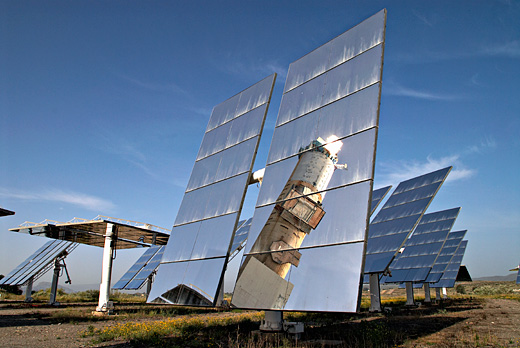
\includegraphics[width=\textwidth]{unnamed (4).png}
Instalación CESA. \cite{PSA1WebSite}

El proyecto CESA-I fue promovido por el Ministerio de Industria y Energía de España e inaugurado en mayo de 1983 para demostrar la viabilidad de las plantas solares de receptor central y para permitir el desarrollo de la tecnología necesaria. En la actualidad CESA-I ya no produce electricidad, sino que se opera, con un alto grado de flexibilidad, como una instalación de ensayo de componentes y subsistemas como helióstatos y receptores solares.
La instalación capta la radiación solar directa por medio de un campo de 300 helióstatos.
La torre es de hormigón y tiene una altura de 80 m, siendo capaz de soportar una carga de 100 toneladas. A lo largo de la torre hay tres niveles de ensayo:
Una cavidad adaptada para su uso como horno solar y ensayo de materiales.
Una cavidad con un banco calorimétrico de ensayo de receptores volumétricos presurizados.
Una instalación de ensayo de receptores volumétricos atmosféricos.
La torre se completa con una grúa en la parte superior con 5 toneladas de capacidad y un elevador montacargas con capacidad para 1.000 kg. \cite{PSA3WebSite}



La instalación SSPS-CRS de 2,5 MWt

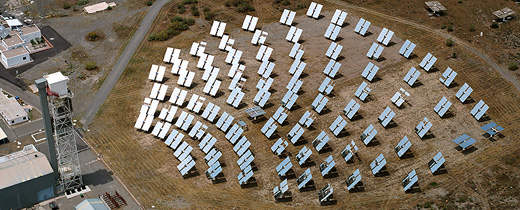
\includegraphics[width=\textwidth]{unnamed (6).png}
Instalación CRS. \cite{PSA2WebSite}

La planta SSPS-CRS fue inaugurada como parte del proyecto SSPS (Small Solar Power Systems) de la Agencia Internacional de la Energía en Septiembre de 1981.
Es una instalación de ensayos dedicada al ensayo de pequeños receptores solares. El campo de helióstatos está formado por 91 unidades, aunque también existe un segundo campo con 20 helióstatos.
El campo de helióstatos CRS ha sido recientemente mejorado con la conversión de todos sus helióstatos en unidades autónomas. En la actualidad, la instalación CRS dispone del primer campo de helióstatos autónomos, que no precisa del uso de zanjas ni cableados.
La torre, de 43 m de altura, es metálica y dispone de tres plataformas de ensayo.
La infraestructura de la torre se completa con una grúa con capacidad para 4.000 kg y un elevador de cremallera con capacidad para 1.000 kg.
Para la caracterización del mapa de flujo de la radiación solar concentrada en ambas torres, se utilizan dos sistemas de medida de flujo: directo e indirecto. El sistema de medida directo consiste en una serie de calorímetros con tiempos de respuesta de microsegundos; están dispuestos en una barra móvil y montada frente a la apertura del receptor. El sistema de medida indirecto consta de una cámara CCD que utiliza un sensor de flujo para la calibración convirtiendo la escala de gris de las imágenes tomadas por la cámara en valores de flujo. \cite{PSA4WebSite}

\end{document}